\documentclass[BoSSSForSolvingConservationLaws.tex]{subfiles}

\begin{document}
\subsection{Coordinate mapping}
\label{sec:CoordinateMapping}
For efficient manipulations on coordinates of DG fields a \emph{coordinate mapping}\coderm{BoSSS.Foundation.CoordinateMapping} is considered which for each coefficient $\hat{u}_{fjn}$ provides an index\coderm{BoSSS.Foundation.CoordinateMapping.LocalUniqueCoordinateIndex()} corresponding to a $1D$ array. This index is called \emph{local unique coordinate index} which is valid on a processor. This local index can be converted\coderm{BoSSS.Foundation.UnsetteledCoordinateMapping.Local2GlobalIndex(...)} to a \emph{global unique coordinate index}\coderm{BoSSS.Foundation.UnsetteledCoordinateMapping.GlobalUniqueCoordinateIndex(...)} that is unique between all processors.
\begin{figure}[h]
\begin{minipage}{0.49\textwidth}
\begin{align*}
&LocalUniqueCoordinateIndex(f,j,n)=\\&j \times \sum_{\lambda=0}^{\Lambda-1} N_{p\lambda-max}+\sum_{\lambda=0}^{f-1}N_{p\lambda-max}+n\\
&0 \le f \le \Lambda-1\\
&0\le j\le J-1\\
&0\le n\le N_{p\lambda} -1
\end{align*}
$\Lambda$ and $J$ are number of fields and cells. $N_{p\lambda}$ is number of basis polynomials for each field $\lambda$ in cell j.
\end{minipage}
\begin{minipage}{0.49\textwidth}
  \begin{center}
  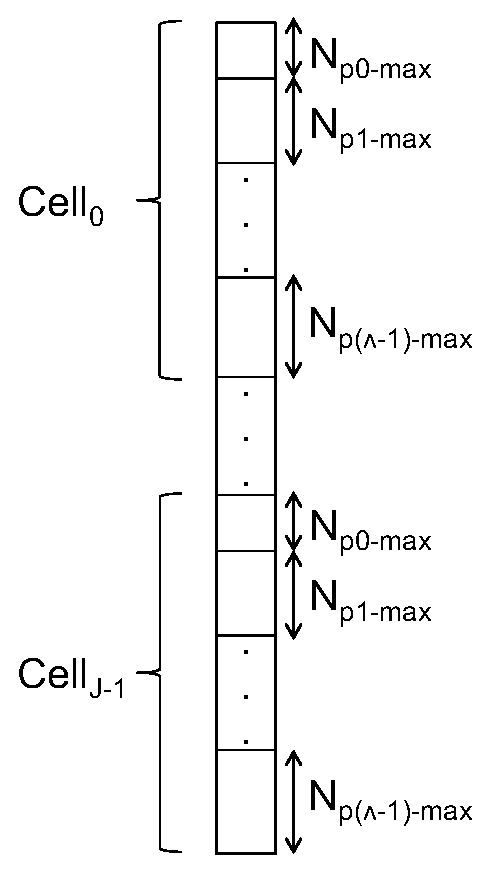
\includegraphics[width=3.5cm]{Figures/CoordinateMapping}
  \end{center}
  \caption{Coordinate mapping}
  \label{fig:CoordinateMapping}
\end{minipage}
\end{figure}

$N_{p\lambda-max}$ is maximum number of basis polynomials\coderm{BoSSS.Foundation.Basis.MaximalLength} of field $\lambda$ over all cells, because a field may be represented by different polynomial degrees in different cells. $\sum_{\lambda=0}^{\Lambda-1}N_{p\lambda-max}$ is called \emph{maximum total number of coordinates per cell}\coderm{BoSSS.Foundation.UnsetteledCoordinateMapping.m\_MaxTotalNoOfCoordinatesPerCell} and the length of the corresponding array of the coordinate mapping is therefore $J\times\sum_{\lambda=0}^{\Lambda-1}N_{p\lambda-max}$.\\
A coordinate mapping is created\coderm{BoSSS.Foundation.CoordinateMapping.CoordinateMapping(...)} by providing a list of DG fields or a list of basis polynomials. The latter case is called \emph{unsettled coordinate mapping}\coderm{BoSSS.Foundation.UnsetteledCoordinateMapping}.
For performing operations like scaling, adding, multiplication by a matrix and so on DG fields a \emph{coordinate vector}\coderm{BoSSS.Foundation.CoordinateVector} must be created from a coordinate mapping. A coordinate vector is basically a list of doubles.

\end{document}

